\subsubsection{Voltaje de rizado}

El cuadro \ref{tab:mediciones-voltaje-rizado} muestra las mediciones de voltaje de rizado para distintas resistencias de carga.

\begin{table}[h!]
    \centering
    \begin{tabular}{|c|c|c|c|}
        \hline
        $V_{rpp}$ (Vpp) & $\Delta V_{rpp}$ (Vpp) & R ($\Omega$) & $\Delta$R ($\Omega$) \\
        \hline
        0.56 & 0.02 & 240 & 12 \\
        0.92 & 0.04 & 110 & 5.5 \\
        1.6 & 0.1 & 60 & 3 \\
        0.12 & 0.01 & 0 & 0 \\
        \hline
    \end{tabular}
    \caption{Mediciones de voltaje de rizado.}
    \label{tab:mediciones-voltaje-rizado}
\end{table}

La figura \ref{fig:voltaje-rizado-110ohm} muestra el voltaje de rizado para una resistencia de 110 $\Omega$.

\begin{figure}[ht]
    \centering
    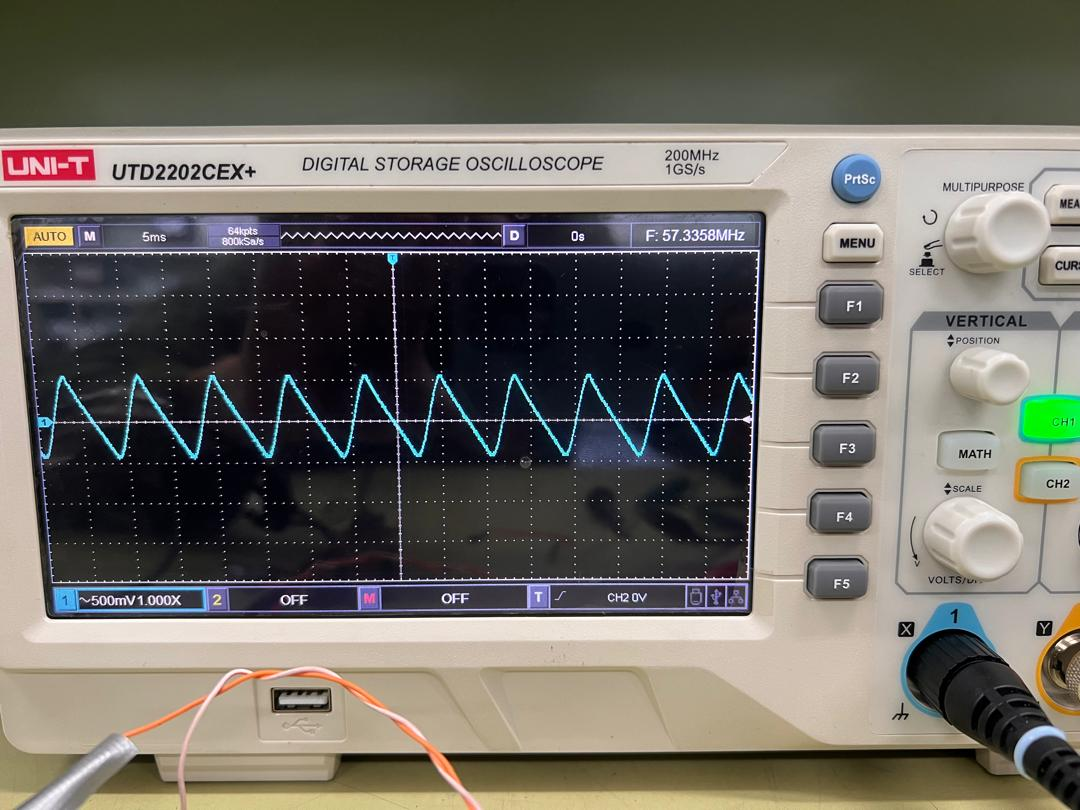
\includegraphics[width=0.5\textwidth]{resultados/voltaje-riso-110ohm.jpg}
    \caption{Voltaje de rizado a 110 $\Omega$.}
    \label{fig:voltaje-rizado-110ohm}
\end{figure}

La figura \ref{fig:voltaje-rizado-240ohm} muestra el voltaje de rizado para una resistencia de 240 $\Omega$.

\begin{figure}[ht]
    \centering
    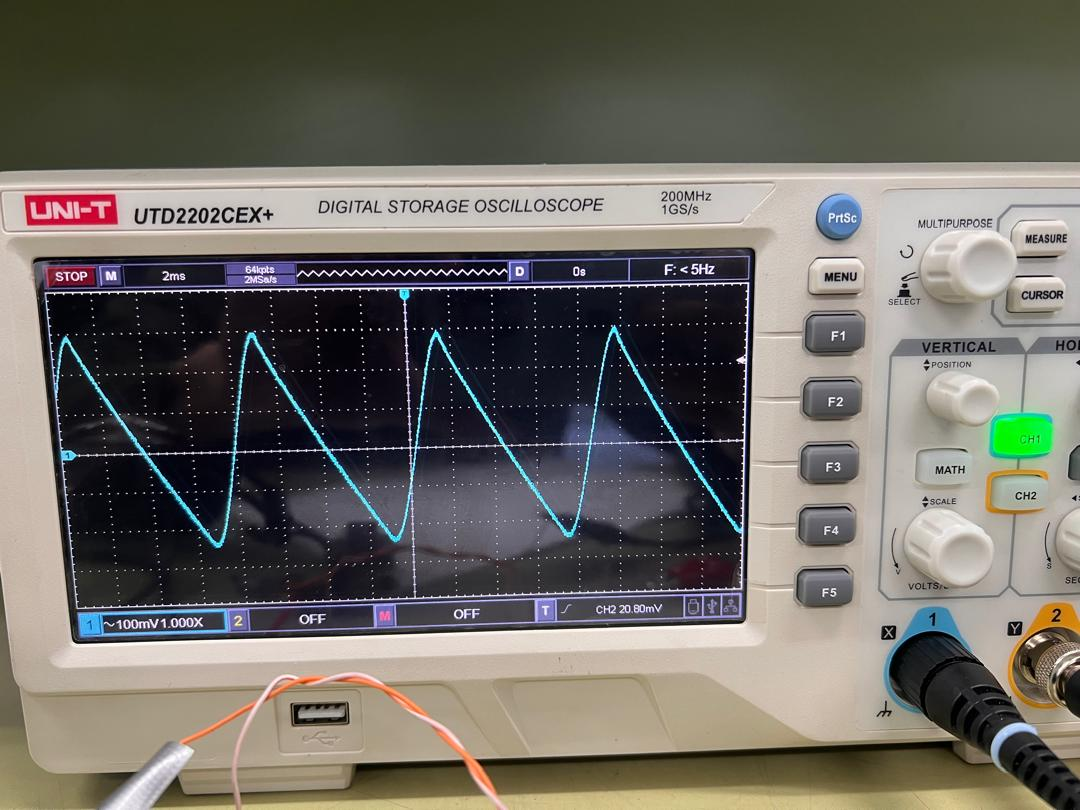
\includegraphics[width=0.5\textwidth]{resultados/voltaje-riso-240ohm.jpg}
    \caption{Voltaje de rizado a 240 $\Omega$.}
    \label{fig:voltaje-rizado-240ohm}
\end{figure}

\FloatBarrier
\subsubsection{Regulación de voltaje Regulador de voltaje de salida fija}

\begin{table}[h!]
    \centering
    \begin{tabular}{|c|c|c|c|c|c|}
        \hline
        $V_{sc}$ (V) & $\Delta V_{sc}$ (V) & $V_{cc}$ (V) & $\Delta V_{cc}$ (V) & Regulación de voltaje (\%) & $\Delta$Regulación de voltaje (\%) \\
        \hline
        5.2 & 0.4 & 5.2 & 0.4 & 0.00 & 10.88 \\
        \hline
    \end{tabular}
    \caption{Mediciones de regulación de voltaje para el regulador de voltaje de salida fija.}
    \label{tab:mediciones-regulacion-voltaje-fija}
\end{table}

\FloatBarrier
\subsubsection{Regulador de salida ajustable}

La tabla \ref{tab:mediciones-regulador-ajustable} muestra las mediciones de voltaje de salida para el regulador ajustable.

\begin{table}[ht]
    \centering
    \begin{tabular}{|c|c|c|}
        \hline
        x & $V_o$ (V) & $\Delta V_o$ (V) \\
        \hline
        1.0 & 15 & 1 \\
        0.5 & 10 & 1 \\
        0.0 & 8 & 1 \\
        \hline
    \end{tabular}
    \caption{Mediciones de voltaje de salida para el regulador ajustable.}
    \label{tab:mediciones-regulador-ajustable}
\end{table}

La tabla \ref{tab:mediciones-amplificador-regulador-ajustable} muestra las mediciones de voltaje en la salida del amplificador en el circuito con el regulador de salida ajustable.

\begin{table}[ht]
    \centering
    \begin{tabular}{|c|c|}
        \hline
        $V_A$ (V) & $\Delta V_A$ (V) \\
        \hline
        3.0 & 1.0 \\
        \hline
    \end{tabular}
    \caption{Medición de voltaje en la salida del amplificador.}
    \label{tab:mediciones-amplificador-regulador-ajustable}
\end{table}

\begin{figure}[ht]
    \centering
    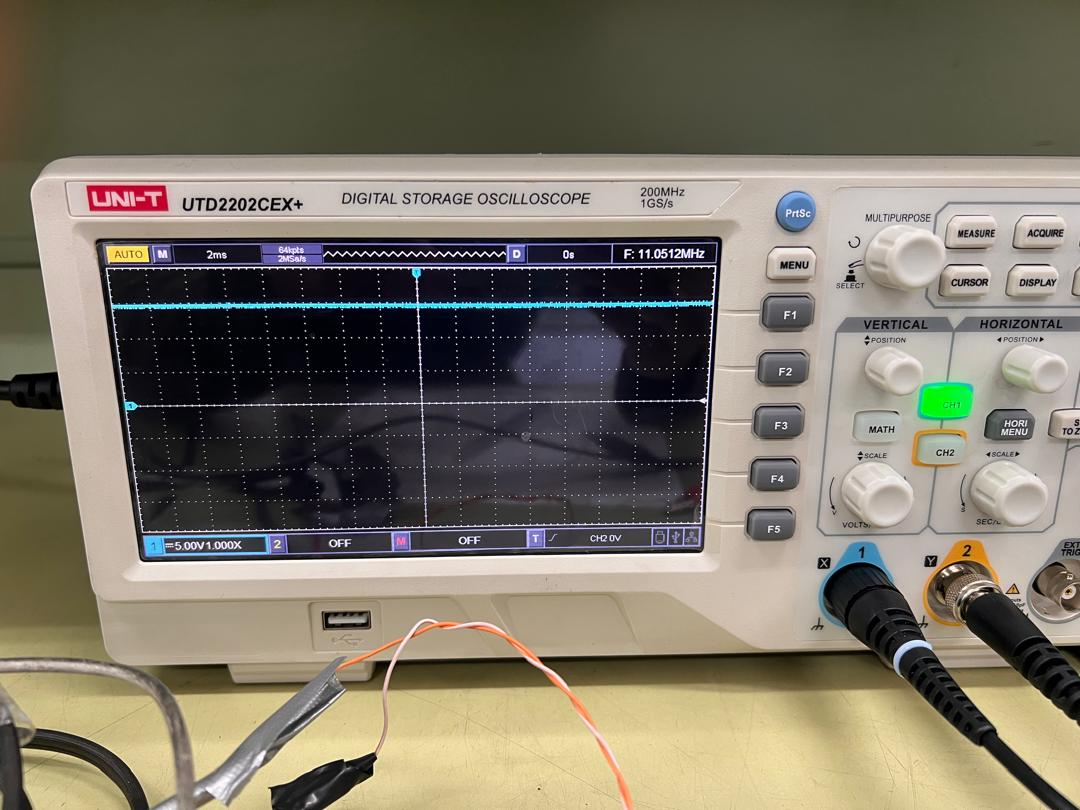
\includegraphics[width=0.5\textwidth]{resultados/voltaje-salida-regulador-variable-x-1.jpg}
    \caption{Voltaje de salida del regulador variable con $x = 1$.}
    \label{fig:voltaje-salida-regulador-variable-x-1}
\end{figure}

\begin{figure}[ht]
    \centering
    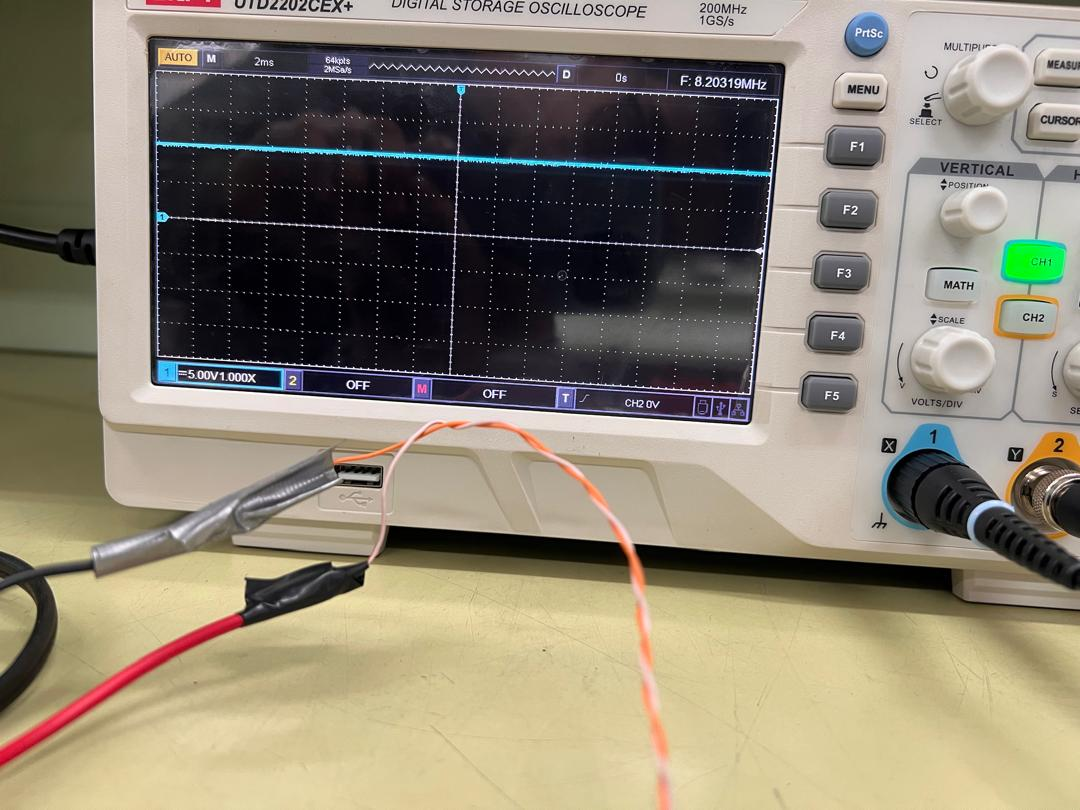
\includegraphics[width=0.5\textwidth]{resultados/voltaje-salida-regulador-variable-x-5.jpg}
    \caption{Voltaje de salida del regulador variable con $x = 0.5$.}
    \label{fig:voltaje-salida-regulador-variable-x-5}
\end{figure}

\FloatBarrier
\subsubsection{Fuente de corriente ajustable}

La tabla \ref{tab:mediciones-fuente-corriente-ajustable} muestra las mediciones de voltaje de salida para la fuente de corriente ajustable con diferentes valores de resistencia de carga.

\begin{table}[ht]
    \centering
    \begin{tabular}{|c|c|c|c|c|}
        \hline
        x & $V_o$ (V) & $\Delta V_o$ (V) & R ($\Omega$) & $\Delta$R ($\Omega$) \\
        \hline
        1.0 & 2.4 & 0.2 & 110 & 5.5 \\
        0.5 & 1.0 & 0.1 & 110 & 5.5 \\
        0.0 & 0.6 & 0.4 & 110 & 5.5 \\
        0.5 & 1.7 & 0.1 & 220 & 11.0 \\
        0.5 & 7.0 & 1.0 & 1000 & 50.0 \\
        0.0 & 4.0 & 1.0 & 1000 & 50.0 \\
        \hline
    \end{tabular}
    \caption{Mediciones de voltaje de salida para la fuente de corriente ajustable.}
    \label{tab:mediciones-fuente-corriente-ajustable}
\end{table}






